%% LyX 2.0.3 created this file.  For more info, see http://www.lyx.org/.
%% Do not edit unless you really know what you are doing.
\documentclass{article}
\usepackage[latin9]{inputenc}
\usepackage{verbatim}
\usepackage{amsmath}
\usepackage{amssymb}
\usepackage{graphicx}
\usepackage[authoryear]{natbib}

\makeatletter
%%%%%%%%%%%%%%%%%%%%%%%%%%%%%% User specified LaTeX commands.
% -----------------------------------------------
% Template for FMA2014
% (based on ISMIR 2010 Template)
% -----------------------------------------------
%
% To compile run:
% pdflatex fma2014template.tex
% bibtex fma2014template
% pdflatex fma2014template.tex (probably twice)
%


\usepackage{fma2014}

% Title.
% ------
\title{Automatic lyrics-to-audio alignment in classical turkish music}

% Single address
% To use with only one author or several with the _same address_
% ---------------
%\oneauthor
% {Author}
% {Affiliation \\ {\tt {author}@fma.edu}}
%
\oneauthor
 {Georgi Dzhambazov, Sertan {\c S}ent\"urk, Xavier Serra}
 {Music Technology Group, Universitat Pompeu Fabra, Barcelona, Spain \\ {\tt \{georgi.dzhambazov,sertan.senturk,xavier.serra\}@upf.edu}}
%
% Two addresses
% --------------
%\twoauthors
%  {First author, Second Author} {Affiliation1 \\ {\tt author1@fma.edu, author2@afm.edu}}
%  {Third author} {Affiliation2 \\ {\tt author3@fma.edu}}
%
% Three addresses
% --------------
%\threeauthors
%  {First author} {Affiliation1 \\ {\tt author1@fma.edu}}
%  {Second author} {Affiliation2 \\ {\tt author2@fma.edu}}
%  {Third author} {Affiliation3 \\ {\tt author3@fma.edu}}





\makeatother

\begin{document}
\maketitle


\section{Introduction}

Lyrics are one of the most important musical components of vocal music.
They convey a story and help create an impression of the song. When
a performance is heard, most listeners will follow the lyrics of the
main vocal melody.

In this perspective, the automatic synchronization between lyrics and
music (also known as lyrics-to-audio alignment) poses a user-demanded
research question. It is applicable to tasks such as automatic karaoke
generation, keyword spotting in singing or the automatic generation
of subtitles for music videos.

By applying a lyrics-to-audio alignment state-of-the-art approach to classical turkish songs,
we aim to outline the research challenges, raised by the musical aspects
peculiar to this music tradition. To this end we compile a dedicated
evaluation corpus. This work is performed in the context of the CompMusic
project \citep{CompMusic2276}, which aims to analyze non-western
music traditions in a culture-specific manner. In this respect,
the corpus is built as well with the intention to be useful for further
music retrieval tasks for the turkish tradition.


\section{Description of classical music of Turkey}

The~\emph{{\c{s}}ark{\i{}}} - the scope of this study - is a
vocal form in the classical repertoire. Typical for it is that vocal
and accompanying instruments follow the same melodic contour in their
corresponding registers with slight melodic variations. However, the
vocal line has usually melodic predominance. This musical interaction
is termed heterophony.

Additionally, the~\emph{{\c{s}}ark{\i{}}} form adheres to a well-defined
verse-refrain-like structure: a ~\emph{{\c{s}}ark{\i{}}} contains
\emph{zemin} (verse), \emph{nakarat} (refrain), \emph{meyan} (second
verse), \emph{nakarat} (refrain) sections, which are preceded by \emph{aranagme}
(an instrumental interlude).

Concerning language, unlike modern Turkish, Ottoman Turkish is characterized by some loanwords
from Arabic and Persian origin. The lyrics language for the ~\emph{{\c{s}}ark{\i{}}}
compositions in our evaluation dataset spans both modern and Ottoman Turkish.


\section{Related work}

To date most of the studies of singing voice in general and the automatic
lyrics-to-audio alignment in particular are focused on western polyphonic
popular music. Many approaches exploit phonetic acoustic features.

An example of such a system \citep{fujihara2011lyricsynchronizer}
relies on a forced alignment scheme and was tested on Japanese popular music. Since the forced alignment technique
was originally developed to carry out the alignment between clean
speech and text, accompanying instruments and non-vocal sections deteriorate
the alignment accuracy. To address this issue, the authors
perform several preprocessing steps of the vocal line: Firstly, the
waveform of the predominant melody is segregated from the polyphonic
signal. Then it is classified into vocal and non-vocal sections. Lastly,
the alignment is run using phonetic features extracted from the vocal-only
signal.

A diametrically different approach is to deploy external information
sources. \citet{muller2007lyrics} uses MIDI files, which are manually
synchronized to lyrics. By performing mapping of timestamps between
an audio recording and a MIDI version of the composition, lyrics are
implicitly aligned to the audio.


\section{Method}

Combining aspects of these two methods, in this work we develop a
system for the automatic synchronization between vocal~\emph{{\c{s}}ark{\i{}}}
recordings and their lyrics. We make use of a modeling scheme based
on phonetic features. Similar to \citet{fujihara2011lyricsynchronizer}
we train a phonetic recognizer, where each phoneme is assigned a hidden
Markov model (HMM).

Furthermore, we exploit a lyrics representation, for which sections
are labeled. Songs are segmented into structural parts through an
external module, which links sections from the musical score to temporal
anchors in the audio. Using a Viterbi forced alignment the system
aligns in a non-linear way the extracted phonetic features to a phoneme
network of trained HMMs.

Figure \ref{Diagram} gives an overview of the layout of the system.

\begin{figure*}
\centerline{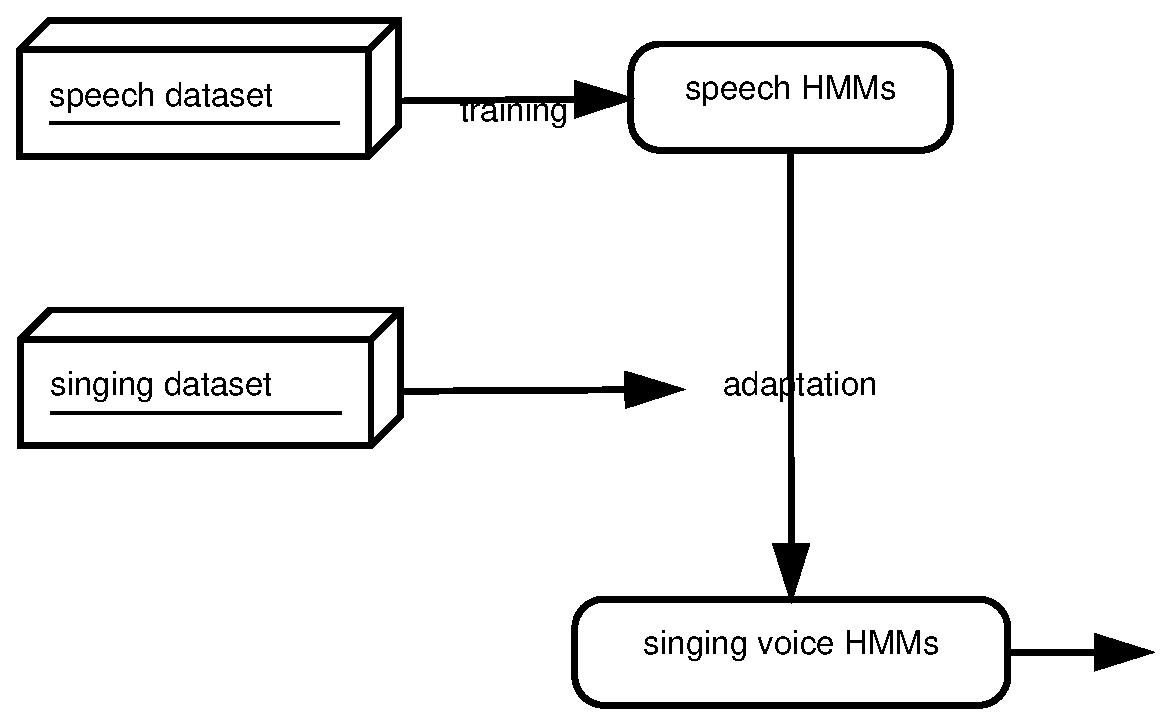
\includegraphics[width=7.9cm]{TrainingWithArrow}\hskip0.05cm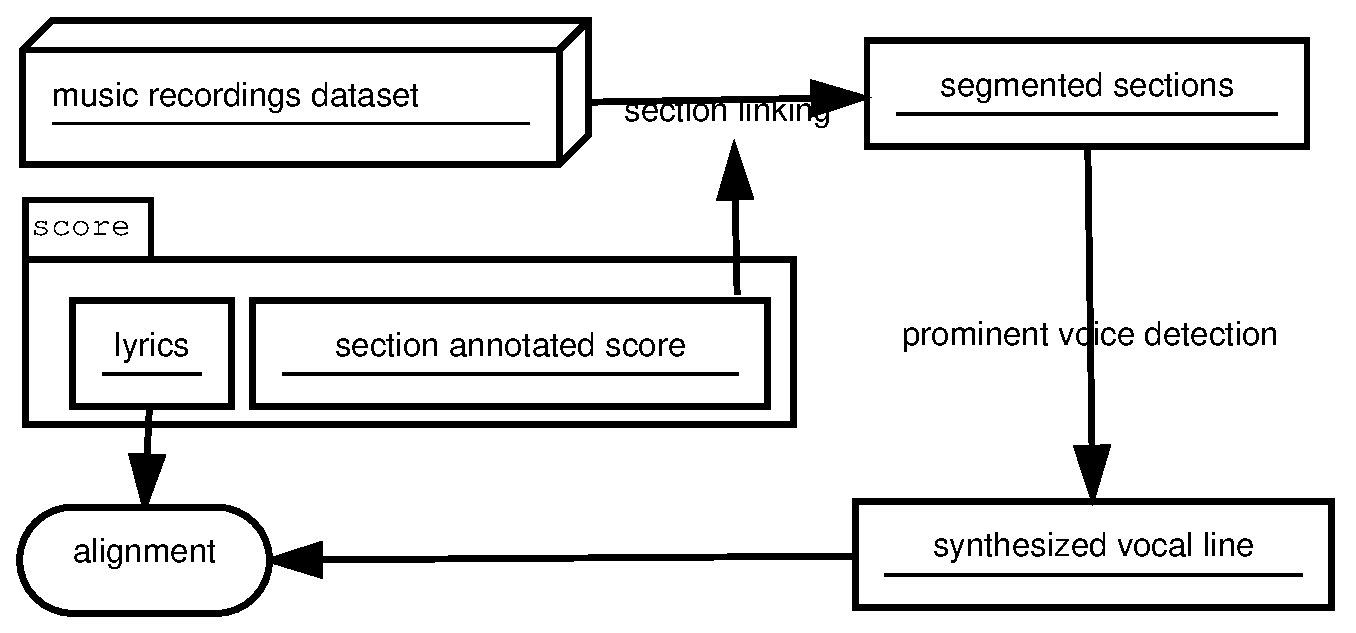
\includegraphics[width=8.5cm]{Alignment}}
\caption{Training steps (on the left) and alignment process (on the right)}


\label{Diagram}

\label{fig:example} 
\end{figure*}



\subsection{Training}

In the absence of annotated data of singing phonemes, we train monophone
models on a big corpus of annotated turkish speech. Later, we adapt
the speech models to match the characteristics of clean singing voice
using a small singing dataset (see Figure \ref{Diagram}).

The acoustic properties (most importantly the formant frequencies)
of spoken phonemes can be induced by the spectral envelope. Thus we
utilize the first 12 mel-frequency cepstral coefficients (MFCCs),
which are known to approximate well the spectral envelope.

An 3-state HMM model for each of 38 turkish phonemes is trained, plus
a silent pause model. For each state a Gaussian distribution is fitted
on the feature vector, which consists of MFCCs and their difference to the previous time instant.


\subsection{Adaptation}

Compared to speech, singing voice possesses different acoustic characteristics.
For example, the pitch of singing voice pertains to the melodic line
in the song, whereas no such dependence holds for speech prosody.

%the fluctuation of fundamental frequency
%(F0) and loudness for a given singer vary more, compared to when she
%is speaking.


The idea of adaptation comes from speaker adaptation and aims to transform
the acoustic space of speaker-independent phoneme models towards the
acoustic characteristics of a particular speaker. \citet{Mesaros96automaticalignment}
have proposed to adapt the speech model instead to singing-voice audio
by means of Maximum likelihood linear regression (MLLR). The MLLR
transform - applied as well in this work - shifts in a linear way
the mean components of the Gaussians of the speech model. This ensures
that after adaptation each state of a phoneme model is more likely to generate
the corresponding phoneme when being sung.


\subsection{Section Linking}

A necessary step to perform alignment is the segmentation of audio
into vocal-containing segments. In the~\emph{{\c{s}}ark{\i{}}}
form each vocal segment is associated with a section (e.g. \emph{nakarat}).
A further challenge is that typically a given performances of a~\emph{{\c{s}}ark{\i{}}}
composition tend to have section repetitions or omissions, which are
not indicated in the score. Thus for each audio recording, prior to
alignment, we utilize a method for detecting structural segments \citep{sertanSectionLinking2014}.
This way we obtain the timestamps of the beginning and ending of each
section in the audio recording (see figure \ref{Diagram}).

% {} The starting and ending points of the sections are explicitly marked
% in the score. The method links the sections in the score to the corresponding
% parts in the audio,  % It generates a synthetic pitch contour from the score, extracts main
% % pitch contour from the audio and matches the two melodic representations.


%% TODO: Accuracy of the section linking part is: Have in mind this as input to our system.


To each segmented vocal section we assign the corresponding lyrical
strophe automatically, because lyric syllables are manually anchored
to notes in the score. The \emph{aranagme} section is discarded.


\subsection{Alignment}

After section detection a source separation step divides the audio
into singing voice and accompanying instruments. The source separation
algorithm applied is described in \citet{durrieu2009main}. To reduce
the negative influence of accompanying instruments, MFCCs are extracted
from the segregated vocal line.

The words from the lyrics are expanded to phonemes based on grapheme-to-phoneme
rules for Turkish%
\begin{comment}
{[}Table 1 of SALOR{]}. 
\end{comment}
. Then the HMMs are concatenated into a phoneme network. An optional
silent pause model, inserted at the end of each word, allows to accommodate
short non-vocal breaks. These presence of such between phrases in
a vocal section are characteristic for ~\emph{{\c{s}}ark{\i{}}}.

The phoneme network is then aligned to the extracted features, resulting
in the time limits of each phoneme.

% vowel harmony? 



\section{Experimental setup}

To train a speech model, perform the adaptation step as well as the
forced alignment, we utilize the HMM Toolkit (HTK).


\subsection{Data}

The speech dataset, used in training, encompasses clean speech covering
60 male and 60 female speakers, totaling to approximately 500 minutes
of speech \citep{Salor2007580}.

The adaptation data consists of 10 vocal-only recordings from classical
turkish singers. The adaptation audio is annotated on phoneme-level,
which enables a model re-estimation in a supervised mode. %
\begin{comment}
vocals are sung with more embellishments. 
\end{comment}


% TODO: tell more about corpus-driven analysis work
The test dataset consists of 15 single-vocal ~\emph{{\c{s}}ark{\i{}}}
performances %
\begin{comment}
of on average 3 minutes each
\end{comment}
. The recordings are selected from a \emph{musicBrainz} collection,
whereas scores are provided in the machine-readable \emph{symbTr}
format \citep{karaosmanouglu2012turkish}%
\footnote{The dataset will be made available on http://compmusic.upf.edu/%
}. These were carefully selected to cover singers of different gender,
different number of accompanying instruments, and different degree
of heterophony.

\begin{comment}
TODO: comment length of sections ranges from ... to .... There are
approximately 9 sections per song. 
\end{comment}



\subsection{Evaluation metric}

Visualization of the word beginning and ending timestamps is a desired
output for subsequent analysis of the lyrics. From this perspective
as an evaluation metric we use the mean of the absolute error of word
timestamps (in seconds).

% TODO: Results section:  Often singers tend to variate the articulation of vocals simultaneously to vibrato effects as a mean of expressivity. This micro-temporal fluctuatins pose a challenge for any singing voice analysis system. 


\bibliographystyle{plainnat}
\bibliography{JabRefCompMusicNon-Lyrics,JabRefLyrics2Audio}

\end{document}
